% This is chapter 2 section 2

\section{Properties of ENP Test}
This section presents an example and four Lemmas to illustrate the properties of the ENP test. 
\subsection{An Example}
Assume three hypotheses given as:
\begin{equation}
  \label{2015jan29a2}
\begin{split}
H_0:\;\;\;\;&X \sim \mathcal{N}(-1, 1)\\
H_1:\;\;\;\;&X \sim \mathcal{N}(0, 1)\\
H_2:\;\;\;\;&X \sim \mathcal{N}(1, 10)
\end{split}
\end{equation}
where $\mathcal{N}(\mu, \epsilon^2)$ denotes a Gaussian PDF with mean $\mu$ and variance $\epsilon^2$. In the following, we compute the ROC surface for the three hypotheses problem \eqref{2015jan29a2}.  
From \eqref{equ: pf and pd} we have  
\begin{equation}
  \begin{split}
	P_{f_1} &= \int_{-\infty}^{\infty}u(f_0(x) - k_1f_1(x) -k_2f_2(x))f_1(x)\mathrm{d}x\\
	P_{f_2} &= \int_{-\infty}^{\infty}u(f_0(x) - k_1f_1(x) -k_2f_2(x))f_2(x)\mathrm{d}x\\
	P_d     &= \int_{-\infty}^{\infty}u(f_0(x) - k_1f_1(x) -k_2f_2(x))f_0(x)\mathrm{d}x\,.
  \end{split}
  \label{2015jan29a1}
\end{equation}

By separately increasing $k_1$ and $k_2$ from $-30$ to $30$ with steps $0.01$, we can calculate the associated $P_{f_1}, P_{f_2}$ and $P_d$ using \eqref{2015jan29a1}. 
Plotting $P_d$ as a function of $P_{f_1}$ and $P_{f_2}$ results in the ROC surface illustrated in Fig. \ref{fig: 2.1} and Fig. \ref{fig: 2.2mar9}. Fig. \ref{fig: 2.1} and Fig. \ref{fig: 2.2mar9} present the ROC surface from different viewpoint. The contour of the ROC surface is given in Fig. \ref{fig: 2.3mar9}. The region enclosed by the two dash lines in Fig. \ref{fig: 2.1}, Fig. \ref{fig: 2.2mar9} and Fig. \ref{fig: 2.3mar9} are the set of points 
achieved by \eqref{2015jan29a1} using non-negative $k_1, k_2$.

It is interesting to observe that under the ENP test framework, not all $(P_{f_1}, P_{f_2})$  ($P_{f_1}, P_{f_2}\in [0, 1]$) values may have an associated $P_d$. This is because for a given $c_1, c_2 \in [0, 1]$, it is possible that no decision rule can satisfy
\[
  P_{f_1} = \int_{\mathcal{S}}f_1(x)\mathrm{d}x =  c_1
\]
and
\[
  P_{f_2} = \int_{\mathcal{S}}f_2(x)\mathrm{d}x = c_2
\]
at the same time. Hence in such case, the corresponding $P_d$ does not exist. 
For example, assume $c_1 = 1$ and $c_2 = 0$. In order to satisfy 
\[
  P_{f_1} = \int_{\mathcal{S}}f_1(x)\mathrm{d}x = 1\,,
\]
the set $\mathcal{S}$  must  be the whole real line, i.e. $\mathcal{S} = (-\infty, \infty)$. However in such case, we have
\[
  P_{f_2} = \int_{\mathcal{S}}f_2(x)\mathrm{d}x = 1 \neq 0
\]
Hence we can see there is no decision rule can satisfy $P_{f_1} = 1$ and $P_{f_2} = 0$ at the same time, and hence the corresponding $P_d$ does not exist.
Recall in the case of binary hypotheses testing (Traditional Neyman Pearson Test), for a given $P_f \in [0, 1]$, there always exists a corresponding $P_d$. 

\begin{figure}[!t]
\centering
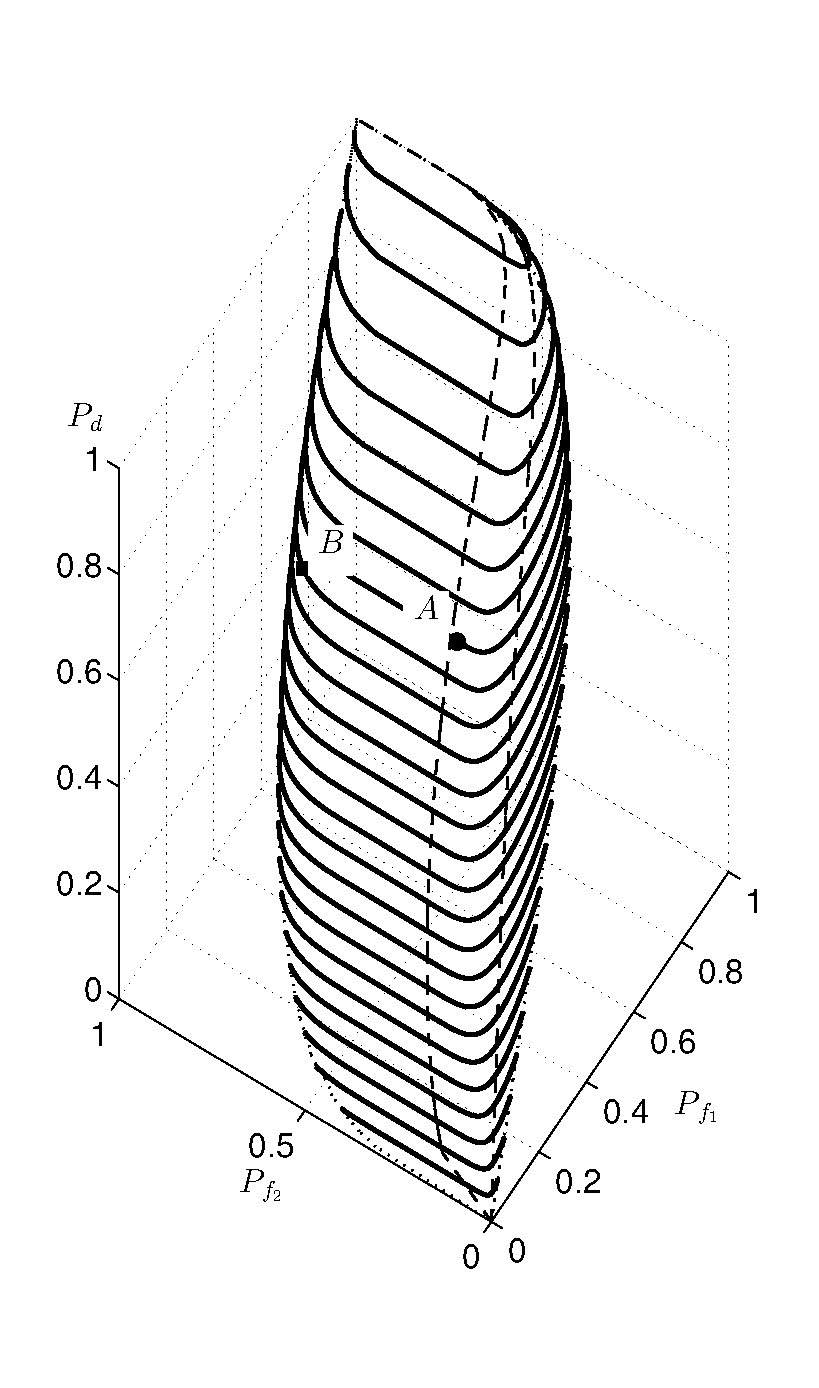
\includegraphics[width = 10cm, height=16cm]{2/ex1.eps}
\caption{The ROC surface for $k_1$, $k_2$ range from $-30$ to $30$ with step $0.01$.}
\label{fig: 2.1}
\end{figure}

\begin{figure}[!t]
\centering
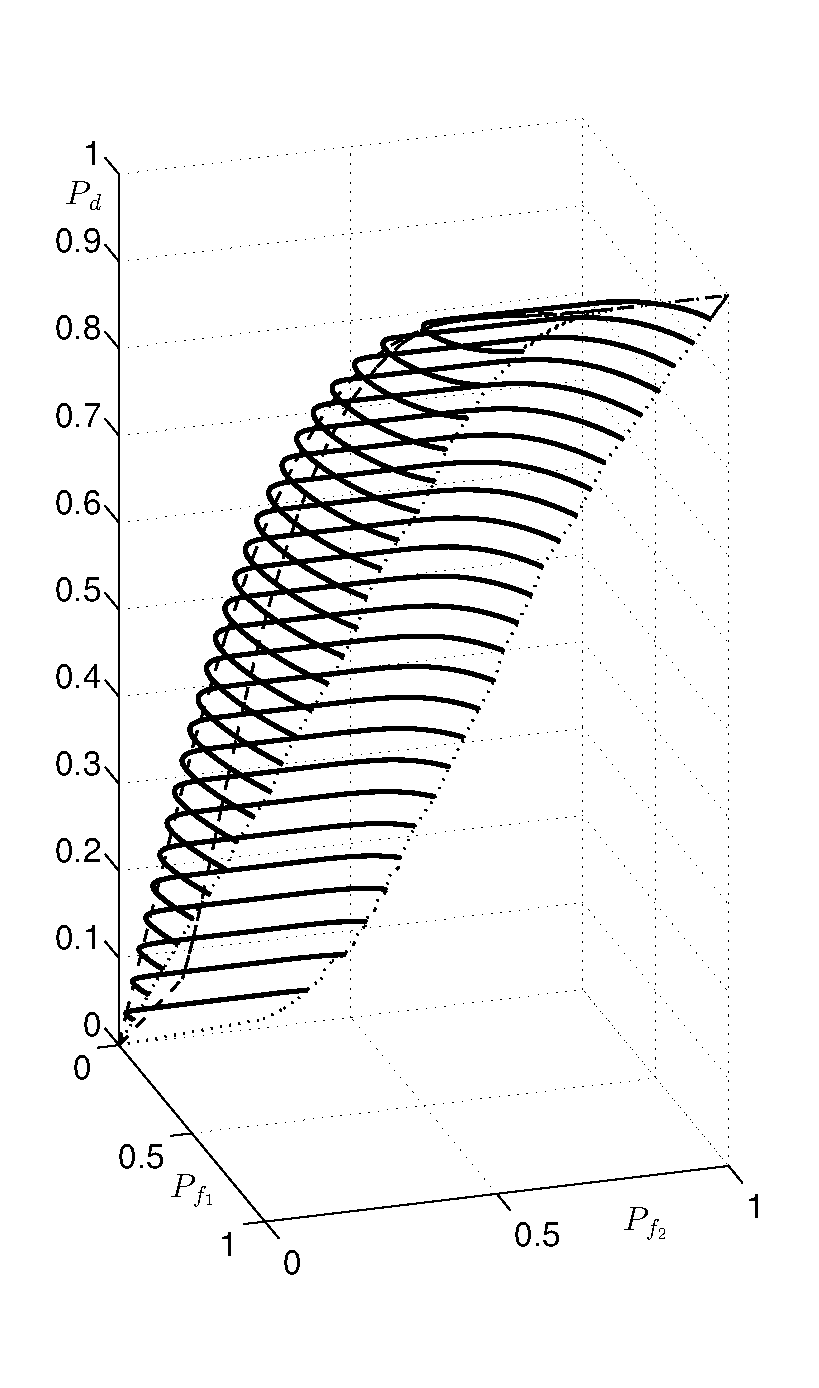
\includegraphics[width = 10cm, height=16cm]{2/ex2.eps}
\caption{The ROC surface for problem \eqref{2015jan29a2}.}
\label{fig: 2.2mar9}
\end{figure}

\begin{figure}[!t]
\centering
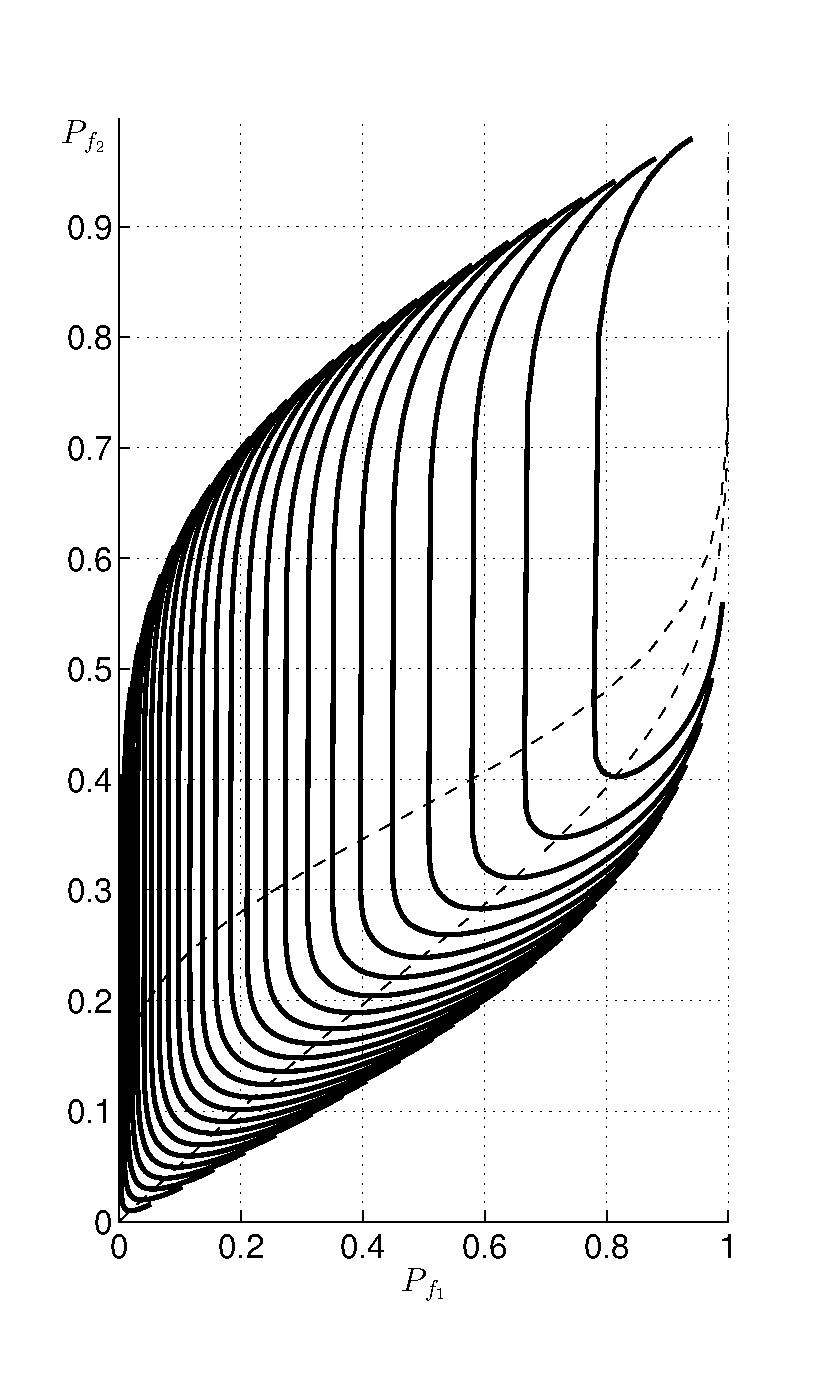
\includegraphics[width = 10cm, height=16cm]{2/ex3.eps}
\caption{The contour for the ROC surface.}
\label{fig: 2.3mar9}
\end{figure}

Now let us consider points $A$ and $B$ on the ROC surface of Fig. \ref{fig: 2.1}, which are marked with '$\bullet$' and '$\blacklozenge$', respectively.  The coordinate of point $A$ is $(P_{f_1}, P_{f_2}, P_d) = (0.350, 0.315, 0.730)$; and the coordinate of point $B$ is  $(P_{f_1}, P_{f_2}, P_d) = (0.355, 0.730, 0.690)$. We can see even through $P_{f_1}$ and $P_{f_2}$ of point $B$ is larger than these of point $A$, the $P_d$ of point $B$ is  smaller than that of point $A$.  
Unlike NP test, where $P_d$ is always non-decreasing with $P_f$, in the case of multiple hypotheses testing (Extended Neyman Pearson Test), $P_d$ is not always a non-decreasing function of  $P_{f_i}$ ($i=1, ..., M$).

Furthermore, we can see in the case of point $B$, the value of $P_d$ is smaller than the value of $P_{f_2}$, i.e. under the ENP framework, $P_d \geq P_{f_i}$  ($i = 1, ..., M$) does not always hold (Qian Zhang arrives at the same conclusion in  \cite{zhang1999design, zhang2000efficient} using a different method). 

\subsection{Four Lemmas for the ENP Test}
Next we presents four lemmas concerning the properties of the ENP test.

%LEMMA 1
\newcommand{\bmu}{\boldsymbol{\mu}}
\typeout{}
\noindent \textbf{Lemma 1}
\noindent \textit{Let $f_0$, $f_1$, ..., $f_M$ be PDFs defined on set $\mathcal{D}$. For given constants $c_1, ..., c_M \in (0, 1)$, let $\mathcal{C}_\delta$ denote a set of decision rules,  such that for $\delta \in \mathcal{C}_\delta$, we have $P_{f_i} \leq c_i$, $i = 1, \cdots, M$. Then:
 among all members of $\mathcal{C}_\delta$ there exists one that maximizes $P_d$.}

\noindent \textbf{PROOF}
Define $\boldsymbol{\mu}_0^T = [\mu_1, ..., \mu_M]$  and  $\mathbf{P}_f^T = [P_{f_1}, P_{f_2}, ..., P_{f_M}]$ that are vectors in an $M$ dimensional Euclidean  space. Let $\bmu^T = [\bmu_0^T, \mu_{M+1}]$ denote a vector in $M+1$ dimensional Euclidean space. 

Let $P_d(\delta)$, $P_{f_i}(\delta)$ denote the $P_d$ and $P_{f_i}$ achieved by using decision rule $\delta$.
%By $\mathbf{A} \leq \mathbf{B}$, $\mathbf{A} = \mathbf{B}$ and  $\mathbf{A} \geq \mathbf{B}$ we mean that every element of $\mathbf{A}$ is no larger than, equal to and no smaller than its corresponding element of $\mathbf{B}$, respectively. 
%By $\mathbf{A} \neq 0$, we mean that every element of $\mathbf{A}$ is not equal to $0$. 

Let us define the set of points in $M+1$ dimensional Euclidean
\begin{equation}
\begin{split}
\label{2015apr28a0}
  \mathcal{N} = \{(\mu_1, \mu_2, ..., \mu_{M+1}) &| \mu_i = \int_{\mathcal{S}}f_i(x)\mathrm{d}x \;\;i=1, ..., M,\\
                                            &  \mu_{M+1}=\int_{\mathcal{S}}f_{0}(x)\mathrm{d}x \;\;\text{ for an $\mathcal{S}$}\}
\end{split}
\end{equation}
We can see that $\mathcal{N}$ is the set of point $(\bmu_0, \mu_{M+1})=(\mathbf{P}_f(\delta), P_d(\delta))$, where $\delta$ is a decision rule. According to \cite{LehmannTest}, set $\mathcal{N}$ is a closed set. We consider one special point in set $\mathcal{N}$. When $\mathcal{S} = \emptyset$, we have $\mu_i = 0$, $i = 1, ..., M+1$, i.e. point $(\mu_1, ..., \mu_{M+1}) = (0, ..., 0)$ is an element of set $\mathcal{N}$.

Define the set of points in $M+1$ dimensional Euclidean Space 
\begin{equation}
\mathcal{P} = \{
(\mu_1, \mu_2, ..., \mu_{M+1}) | \bmu_0 \in [0^M, \mathbf{c}], \mu_{M+1} \in [0, 1]
\}\,.
\end{equation}
Clearly set $\mathcal{P}$ is also a closed set and point $(\mu_1, ..., \mu_{M+1}) = (0, ..., 0)$ is also an element  of set $\mathcal{P}$.


Let $\mathcal{K} = \mathcal{N} \cap \mathcal{P}$, i.e.
\begin{equation}
\label{apr14a0}
\mathcal{K} = \{
(\mu_1, \mu_2, ..., \mu_{M+1}) | (\bmu_0, \mu_{M+1}) \in \mathcal{N} \text{ and } \bmu_0 \in [0^M, \mathbf{c}], \mu_{M+1} \in [0, 1]
\}\,.
\end{equation}

Point $(\mu_1, ..., \mu_{M+1}) = (0, ..., 0)$ belongs to both $\mathcal{N}$ and $\mathcal{P}$, hence it belongs to set $\mathcal{K}$. This suggests set $\mathcal{K}$ is not an empty set.

As both $\mathcal{N}$ and $\mathcal{K}$ are closed set, $\mathcal{K}$ is also closed. Besides that, for any point  $(\mu_1, \mu_2, ..., \mu_{M+1}) \in \mathcal{K}$, we have $\mu_i \in [0, c_i]$ and $\mu_{M+1} \in [0,1]$. Thus we can conclude set $\mathcal{K}$ is a bounded set. As $\mathcal{K}$ is a closed and bounded set in $M+1$ Euclidean Space, it is compact \cite{johnsonbaugh2012foundations}. 

Define function $f: \mathbf{R^{M+1}} \rightarrow \mathbf{R}$ as
\begin{equation}
f(\mu_1, \mu_2, ..., \mu_{M+1}) = \mu_{M+1}\,.
\end{equation}

It is easy to see $f$ is a continuous function. According to \cite{johnsonbaugh2012foundations}, $f$ attains a maximum and minimum value on set $\mathcal{K}$. 
Without losing generality, assume $f(\bmu^0)  = \mu_{M+1}^0$ (where $\bmu^0 = (\mu_1^0, \cdots, \mu_{M+1}^0)$ and $\bmu^0 \in \mathcal{K}$) achieve this maximum value. 
Since $\bmu^0 \in \mathcal{K}$ and $\mathcal{K}  \subseteq  \mathcal{N}$, from the definition of $\mathcal{N}$, there exists a decision rule $\delta^\ast$ such that $(\mathbf{P}_{f}(\delta^\ast), P_d(\delta^\ast)) = \bmu^0$.  
Furthermore, since $\bmu^0 \in \mathcal{K} $, from the definition of $\mathcal{K}$ we know $\mathbf{P}_{f}(\delta^\ast) \leq \mathbf{c}$, 
i.e. $\delta^\ast$ is a member of $\mathcal{C}_\delta$. 
Let $\delta' $ be another decision rule in set $\mathcal{C}_\delta$, we have $(\mathbf{P}_f(\delta'), P_d(\delta')) \in \mathcal{N}$ and $(\mathbf{P}_f(\delta'), P_d(\delta')) \in \mathcal{P}$, i.e. $(\mathbf{P}_f(\delta'), P_d(\delta')) \in \mathcal{K}$.
Since $f(\bmu^0) = \mu_{M+1}^0$ achieves the maximum value for $\bmu \in \mathcal{K}$, we have
$f((\mathbf{P}_f(\delta'), P_d(\delta')))  = P_d(\delta') \leq  f(\bmu^0) = \mu_{M+1}^0 =  P_d(\delta^\ast)$, i.e. $\delta^\ast$ maximize $P_d$ among all members of $\mathcal{C}_\delta$.

Q.E.D.


\noindent \textbf{Lemma 2}
\noindent \textit{
Let $f_0$, $f_1$, ..., $f_M$ be PDFs defined on set $\mathcal{D}$. For given constants $c_1, ..., c_M \in (0, 1)$, let $\mathcal{C}_\delta$ denote a set of decision rules,  such that for any $\delta \in \mathcal{C}_\delta$, we have $P_{f_i} \leq c_i$, $i = 1, \cdots, M$.
%No. 1
%\\\textnormal{(\rmnum{1})} Among all members of $\mathcal{C}_\mathcal{S}$ there exists one that maximizes $P_d$.
%No.2
If  $\delta^{\ast}$ is a member of $\mathcal{C}_\delta$ and it maximize $P_d$ among all members of $\mathcal{C}_\delta$, then there exists non-negative constants $k_1, ..., k_M$ such that $\delta^\ast$ can be written in form of  
\begin{equation}
f_0(x) \substack{H_0 \\ \geq \\ < \\ \bar{H}_0} \sum_{j=1}^{M}k_jf_j(x)
\end{equation}
Moreover, under decision rule $\delta^\ast$ if  $P_{f_i} < c_i$, then $k_i = 0$. 
}

In \cite{zhang1999design, zhang2000efficient} Qian Zhang also arrives at the conclusion that if $P_{f_i} < c_i$ then $k_i = 0$, through analyzing the change of $P_d$ with respect to $k_i$ (he shows if $P_{f_i} < c_i$ and $k_i > 0$, then the $P_d$ can be further increased through adjusting the value of $k_i$). In the following we will prove \textbf{Lemma 2} using a mathematical method such that used in \cite{LehmannTest, dantzig1951fundamental} to prove the ENP Lemma (\rmnum{4}).

\noindent\textbf{PROOF}
We start by defining some notations for easy presentation.
Define $\mathbf{c}^T = [c_1, c_2, ..., c_M]$ and  $\mathbf{k}^T = [k_1, k_2, ..., k_M]$ that are vectors in an $M$ dimensional Euclidean  space. Let $\bmu^T = [\bmu_0^T, \mu_{M+1}]$ denote a vector in $M+1$ dimensional Euclidean space. 

Let $F(\boldsymbol{\mu}_0)$ denote the largest $P_d$ under the constraints $P_{f_i} = \mu_i\;\;i = 1, ..., M$.
Let $G(\boldsymbol{\mu}_0)$ denote the largest $P_d$ under the constraints $P_{f_i} \leq \mu_i\;\;i = 1, ..., M$.
By $\mathbf{A} \leq \mathbf{B}$, $\mathbf{A} = \mathbf{B}$ and  $\mathbf{A} \geq \mathbf{B}$ we mean that every element of $\mathbf{A}$ is no larger than, equal to and no smaller than its corresponding element of $\mathbf{B}$, respectively. 
By $\mathbf{A} \neq 0$, we mean that every element of $\mathbf{A}$ is not equal to $0$. 
Let $G'$ denote the hyper surface in an $M+1$ dimensional Euclidean Space defined by 
\begin{equation}
 \label{def: G'}
 G' = \{(\bmu_0, \mu_{M+1})  | \bmu_0 \in [0, 1]^M, \mu_{M+1}= G(\bmu_0) \}\,.
\end{equation}
Let $G_s$ denote the set of points in an $M+1$ Euclidean space defined as 
\begin{equation}
  \label{2015feb16n1}
G_s =  \{(\boldsymbol{\mu}_0, \mu_{M+1}) | \boldsymbol{\mu}_0\in [0, 1]^M, \mu_{M+1} \in [0, G(\mathbf{\bmu_0})]
    \}\,.
  \end{equation}
  From \eqref{def: G'} and \eqref{2015feb16n1}, it can be seen $G' \in G_s$. Fig. \ref{fig: feb18} depicts the relationship between $G'$ and $G_s$ when $M=2$. In Fig. \ref{fig: feb18}, $G'$ is the surface enclosed by curve $\stackrel\frown{AC}$, curve $\stackrel\frown{AD}$, segment $\overline{OC}$ and segment $\overline{OD}$. Set $G_s$ is the space enclosed by plane $ABC$, plane $ABD$, plane $COD$ and surface $G'$.  

\begin{figure}[!t]
\centering
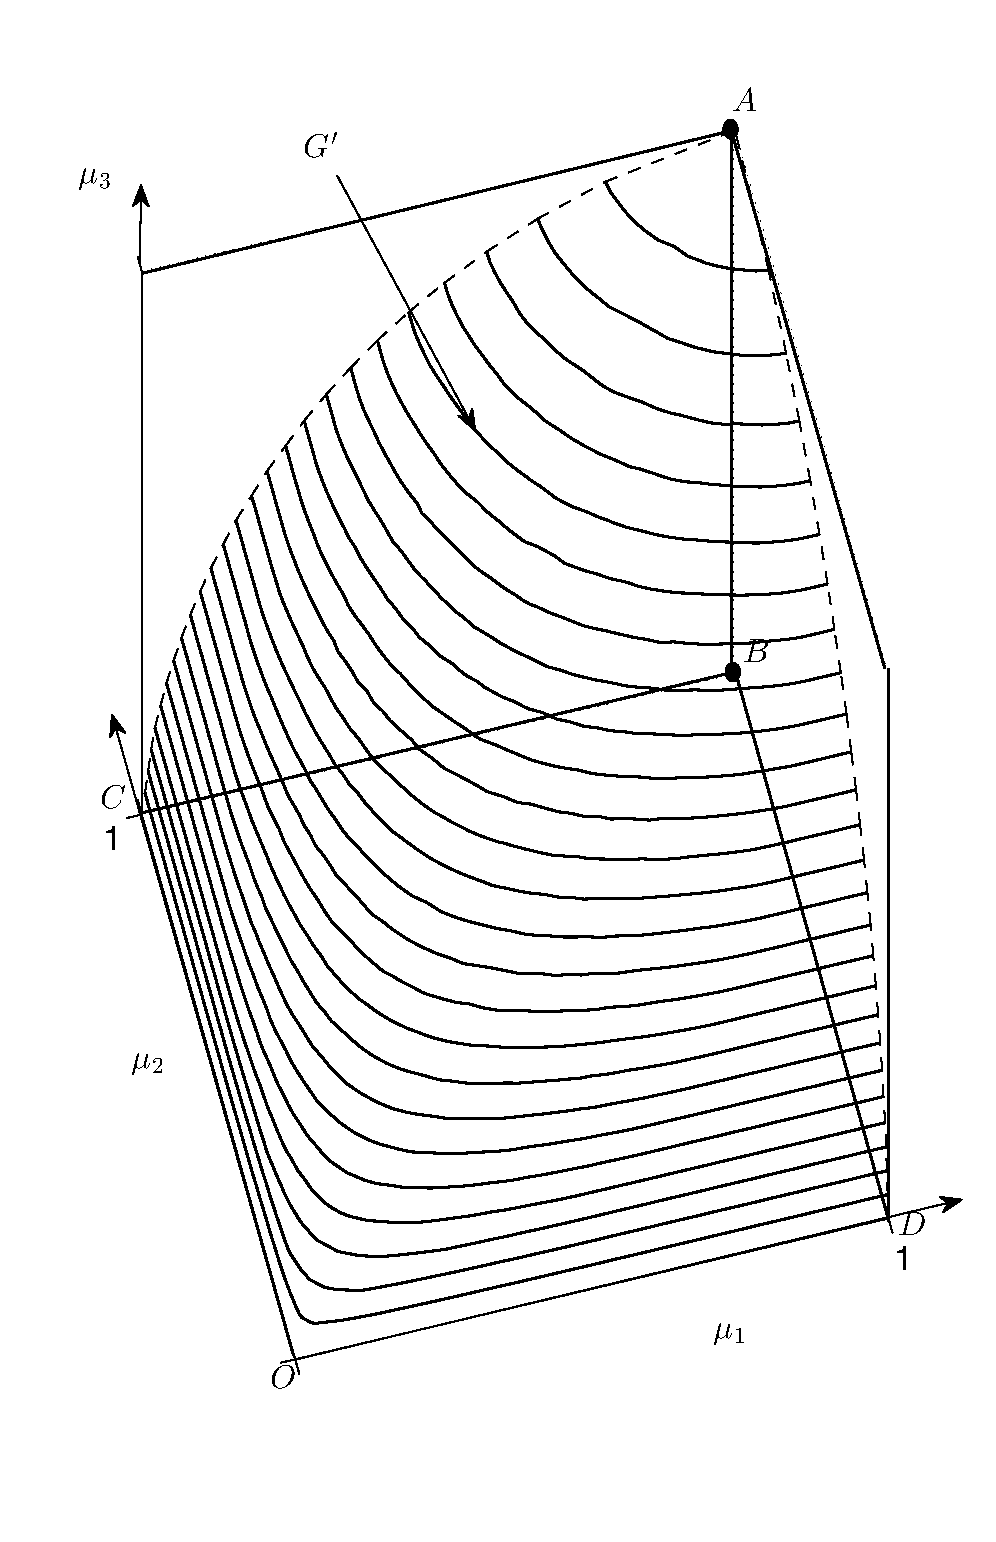
\includegraphics[width = 12cm, height=16cm]{2/example_pic.eps}
\caption{Relationship between $G'$ and $G_s$}
\label{fig: feb18}
\end{figure}
As we defined in \eqref{2015apr28a0}, $\mathcal{N}$ is the set of point $(\bmu_0, \mu_{M+1})=(\mathbf{P}_f(\delta), P_d(\delta))$, where $\delta$ is a decision rule.
From the definition of $\mathcal{N}$ and $F(\bmu_0)$ we can conclude that for a point $(\bmu_0, \mu_{M+1}) \in \mathcal{N}$, we have $\mu_{M+1} \leq F(\bmu_0)$. 
To see this, assume $\mu_{M+1} > F(\bmu_0)$. Then there is a decision rule $\delta$ such that $P_{f_i}(\delta) = \mu_i$ ($i=1, ..., M$) and $P_d(\delta) > F(\bmu_0)$. This is contradictory to the definition of $F(\bmu_0)$. 

The whole proof consists of the following parts: first we prove $G(\boldsymbol{\mu}_0)$ is a convex, non-decreasing function, and when $\boldsymbol{\mu}_0 > 0$, $G(\boldsymbol{\mu}_0) > 0$;
secondly it will be shown that $G_s$ is a convex set and $\mathcal{N} \subseteq G_s$; 
after that we will illustrate that for a point $(\mu_1^0, \mu_2^0, ..., \mu_{M+1}^0) \in G'$, there exists a non-negative $\mathbf{k}$ such that 
\[
\mu_{M+1} - \sum_{i=1}^{M}k_i\mu_i \leq \mu_{M+1}^0 - \sum_{i=1}^{M}k_i\mu_i^0
\]
holds for point $(\mu_1, \mu_2, ..., \mu_{M+1}) \in G_s$;
at the end, we will show for $\mathbf{c} \in (0, 1)$, there exists a non-negative $\mathbf{k}$ such that the optimal decision rule to achieve the largest $P_d$ under constraint $\mathbf{P}_f \leq \mathbf{c}$ can be written in the form
\[
f_0(x) \substack{H_0 \\ > \\ < \\ \bar{H}_0} \sum_{i=1}^{M}k_if_i(x)\,.
\]

Firstly we will prove $G(\bmu_0)$ is a convex non-decreasing function in each variable $\mu_i$, $i = 1, \cdots, M$.
 Let $\boldsymbol{\mu}^1$ and  $\boldsymbol{\mu}^2$ be two points on $G'$ with coordinates $(\boldsymbol{\mu}^1_0, \mu_{M+1}^1)$ and $(\boldsymbol{\mu}^2_0, \mu_{M+1}^2)$, i.e. $\mu_{M+1}^1 = G(\boldsymbol{\mu}_0^1)$ and $\mu_{M+1}^2 = G(\boldsymbol{\mu}_0^2)$. Let $\delta_1$ be a decision rule which can achieve the largest $P_d$ under the constraint $\mathbf{P}_f \leq \boldsymbol{\mu}_0^1$ and $\delta_2$ be a decision rule which can achieve the largest $P_d$ under the constraint $\mathbf{P}_{f} \leq \boldsymbol{\mu}_0^2$. Thus we can see 
 \begin{subequations}
\begin{align}
&\mu_{M+1}^1 = P_d(\delta^1) = G(\boldsymbol{\mu}_0^1)\\
&\mu_{M+1}^2 = P_d(\delta^2)=G(\boldsymbol{\mu}_0^1)\\
&\mathbf{P}_f(\delta^1) \leq \boldsymbol{\mu}^1_0\\
&\mathbf{P}_f(\delta^2) \leq \boldsymbol{\mu}^2_0
\end{align}
 \end{subequations}
 
Construct a new randomized test $\delta^3$, where $\delta^1$ and $\delta^2$ are used with equal probability. With decision rule $\delta^3$, we have 
\begin{subequations}
\begin{align}
\label{1120night1}
&P_d(\delta^3) = 0.5P_d(\delta^1)+0.5P_d(\delta^2) = 0.5G(\bmu_0^1) + 0.5G(\bmu_0^2)\\
&\mathbf{P}_{f}(\delta^3) = 0.5\mathbf{P}_f(\delta^1)+0.5\mathbf{P}_f(\delta^2) \leq 0.5\boldsymbol{\mu}^1_0 + 0.5\boldsymbol{\mu}^2_0
\end{align}
\end{subequations}
Let $\delta'$ denote the optimal decision rule for 
 \begin{equation}
 \begin{split}
 \label{1120t}
 \max&\;\;\;\;P_d\\
 \text{s.t.}&\;\;\;\;\mathbf{P}_f \leq 0.5\boldsymbol{\mu}^1_0 + 0.5\boldsymbol{\mu}^2_0
 \end{split}
 \end{equation}
then obviously $P_d(\delta') \geq P_d(\delta^3)$ (otherwise $\delta'$ cannot be the optimal decision rule for \eqref{1120t}). Since $P_d = G(0.5\boldsymbol{\mu}^1_0 + 0.5\boldsymbol{\mu}^2_0)$, we have  
\begin{equation}
\label{1120t2}
G(0.5\boldsymbol{\mu}^1_0 + 0.5\boldsymbol{\mu}^2_0) \geq  P_d(\delta^3).
\end{equation}
Substituting \eqref{1120night1} in \eqref{1120t2} results in
\begin{equation}
\label{1120t3}
G(0.5\boldsymbol{\mu}^1_0 + 0.5\boldsymbol{\mu}^2_0) \geq 0.5 G(\boldsymbol{\mu}^1_0)+ 0.5 G(\boldsymbol{\mu}^2_0)\,.
\end{equation}
showing that  $G(\bmu_0)$ is a convex function for $\bmu_0 \in [0, 1]^M$.

According to the definition of $G(\bmu_0)$, when $\mu_i$ increases, the false alarm constraints are relaxed, 
so the value of $G(\bmu_0)$ will either remain the same or increase. 
This suggests $G(\bmu_0)$ is a non-decreasing function of $\bmu_0$. 
This is not contradictory with the conclusion that 
$P_d$ is not always increasing with $P_{f_i}\;\;(i=1, 2, \cdots, M)$  (we arrived at this conclusion in Chapter 2 section 1.1 on page 12).  This is because $\bmu_0$ is not the probability of false alarms but rather the constraints of the probability of false alarm. 

Next we will show when $\boldsymbol{\mu}_0 > 0^M$, then $G(\boldsymbol{\mu}_0)$ is strictly larger than zero.
Let $\delta^\ast$ be the optimal decision rule for $\bmu_0$. By optimal  we mean that this decision rule provides the largest $P_d$ under the constraints $\mathbf{P}_f \leq \bmu_0$, i.e. $P_d(\delta^\ast) = G(\bmu_0)$. Consider two decision rule $\delta^1$ and $\delta^2$ defined as 
\begin{equation}
  \label{2015feb09a4}
  \delta^1:\;\; \begin{cases}
    & \text{ $H_0$ if } x \in \emptyset \\
    & \text{ $\bar{H}_0$ if } x \in \mathcal{D}
  \end{cases}
\end{equation}
and
\begin{equation}
  \label{2015feb09a5}
  \delta^2:\;\; \begin{cases}
    & \text{ $H_0$ if } x \in \mathcal{D} \\
    & \text{ $\bar{H}_0$ if } x \in \emptyset
  \end{cases}
\end{equation}

From \eqref{2015feb09a4} and \eqref{2015feb09a5} we can see the $P_d$ and $P_{f_i}$ under under decision rule $\delta^1$ and $\delta^2$ can be written as
\begin{equation}
  P_d(\delta^1) = \int_{\emptyset}f_0(x)\mathrm{d}x = 0
\end{equation}
\begin{equation}
    P_{f_i}(\delta^1) = \int_{\emptyset}f_i(x)\mathrm{d}x = 0
\end{equation}
\begin{equation}
    P_d(\delta^2) = \int_{\mathcal{D}}f_0(x)\mathrm{d}x = 1
\end{equation}
\begin{equation}
    P_{f_i}(\delta^2) = \int_{\mathcal{D}}f_i(x)\mathrm{d}x = 1
\end{equation}

Let $\mu_{min} = \min(\mu_1, \mu_2, \cdots, \mu_M)$. Since $\bmu_0 > 0^M$, we know $\mu_i > 0$ for $i = 1, \cdots, M$. Thus we have $\min(\mu_1, \cdots, \mu_M) > 0$, i.e. $\mu_{min} > 0$. Construct a new randomized test $\delta^3$ where $\delta^1$ and $\delta^2$ are used with probability $1 - \mu_{min} $ and $\mu_{min}$. With decision rule $\delta^3$ we have
\begin{equation}
  P_d(\delta^3) = (1 - \mu_{min})P_d(\delta^1) + \mu_{min}P_d(\delta^2) = \mu_{min} > 0
\end{equation}
\begin{equation}
  P_{f_i}(\delta^3) = (1 - \mu_{min})P_{f_i}(\delta^1) + \mu_{min}P_{f_i}(\delta^2) = \mu_{min} \leq \mu_i \;\;\;\;(i = 1, 2, \cdots, M)
\end{equation}

Hence we can see by using $\delta^3$ we have
\[
  \mathbf{P}_f(\delta^3) \leq \bmu_0\,.
\]
Since $\delta^\ast $ is the optimal decision rule for $\bmu_0$, we can conclude $P_d(\delta^\ast) \geq  P_d(\delta^3) = \mu_{min} >  0$. Since $G(\bmu_0) = P_d(\delta^\ast)$, we can conclude $G(\bmu_0) > 0$ when $\bmu_0 > 0 $. 


In the following, we consider the property of $G_s$. First we will prove that $G_s$ is a convex set. 
Let $\boldsymbol{\mu}^1$ and  $\boldsymbol{\mu}^2$ be two points that belong to $G_s$ with coordinates $(\boldsymbol{\mu}^1_0, \mu_{M+1}^1)$ and $(\boldsymbol{\mu}^2_0, \mu_{M+1}^2)$. According to the definition of $G_s$, we have 
\begin{subequations}
\label{1120t4}
\begin{align}
\label{1120night6}
&0^M \leq \bmu_0^1 \leq 1^M\\
\label{1120night7}
&0^M \leq \boldsymbol{\mu}^2_0 \leq 1^M\\
\label{1120night3}
&0 \leq \mu_{M+1}^1 \leq G(\boldsymbol{\mu}_0^1)\\
\label{1120night4}
&0 \leq \mu_{M+1}^2 \leq G(\boldsymbol{\mu}_0^2)
\end{align}
\end{subequations}

Let $\boldsymbol{\mu}^3$ be the middle point between $\boldsymbol{\mu}^1$ and $\boldsymbol{\mu}^2$ with coordinate $(\bmu_0^3, \mu_{M+1}^3)$, where  
\begin{subequations}
\label{1120t5}
\begin{align}
\label{1120night5}
\bmu_0^3 &= 0.5\boldsymbol{\mu}_0^1 + 0.5 \boldsymbol{\mu}_0^2\\
\label{1120night2}
\mu_{M+1}^3 &= 0.5 \mu_{M+1}^1 + 0.5 \mu_{M+1}^2
\end{align}
\end{subequations}
In the following, we will show $\bmu^3 \in G_s$.  
From \eqref{1120night6}, \eqref{1120night7} and \eqref{1120night5} we can see that
\begin{equation}
\label{equ: 1120n1}
\bmu_0^3 \in [0, 1]^M
\end{equation}
Substituting \eqref{1120night3} \eqref{1120night4} into \eqref{1120night2}, we have
\begin{equation}
  \label{equ:2015feb1a}
0 \leq \mu_{M+1}^3 \leq 0.5 G( \bmu_0^1) + 0.5G(\bmu_0^2)\,.
\end{equation} 
Using \eqref{1120t3} and \eqref{1120night5} with \eqref{equ:2015feb1a} gives,
\begin{equation}
\label{equ: 1120n}
0 \leq \mu_{M+1}^3 \leq G(0.5 \bmu_0^1 + 0.5\bmu_0^2) = G(\bmu_0^3)\,.
\end{equation}
From \eqref{equ: 1120n} and \eqref{equ: 1120n1}, it follows that  
 $\bmu^3 \in G_s$, showing that $G_s$  is a convex set.  

Next we prove $\mathcal{N} \subseteq G_s$. We need to show that if  $\forall (\mu_1, ..., \mu_{M+1}) \in \mathcal{N}$, then this point also belongs to $G_s$.
Assume $(\mu_1^N, ..., \mu_{M+1}^N)$ is a point in $\mathcal{N}$. 
In previous discussion, it has been shown $\mu_i^N \in [0, 1]$ ($i = 1, ..., M$) and $\mu_{M+1}^N \in [0, F(\bmu_0^N)]$, where $\bmu_0^N = [\mu_1^N, ..., \mu_M^N]$. 
According to the definition of $G(\bmu_0)$ and $F(\bmu_0)$, we can conclude $G(\bmu_0^N) \geq F(\bmu_0^N)$. 
This implies $\mu_{M+1}^N \in [0, G(\bmu_0^N)]$ and we have  
\begin{equation}
\begin{split}
&\mu_i^N \in [0, 1]\;\;\;\;(i=1, 2, ..., M)\\
&\mu_{M+1}^N \in [0, G(\bmu_0^N)]
\end{split}
\end{equation}
showing that point $(\mu_1^N, ..., \mu_{M+1}^N)$ also belongs to set $G_s$.
Hence we proved $\mathcal{N} \subseteq G_s$. 

In the following we will show for a point $(\mu_1^0, \mu_2^0, ..., \mu_{M+1}^0)$ that belongs to $G'$ ($\mu_i^0 \in (0, 1), i = 1, 2, ..., M$), there exists a non-negative $\mathbf{k}$ such that  
\[
\mu_{M+1} - \sum_{i=1}^{M}k_i\mu_i \leq \mu_{M+1}^0 - \sum_{i=1}^{M}k_i\mu_i^0
\]
holds for any $(\mu_1, \mu_2, ..., \mu_{M+1}) \in G_s$. 
Assume $(\mu_0^0, \mu_1^0, ..., \mu_{M+1}^0)$ is a point on the $G'$ surface, i.e. $\mu_{M+1}^0 = G(\bmu_0^0)$, where $\bmu_0^0 = [\mu_1^0, ..., \mu_{M}^0]$. 
Also we assume $\mu_1^0, \mu_2^0, ..., \mu_M^0 \in (0, 1)$. 
According to the definition of $G_s$, for any positive $\epsilon$, point $(\mu_0^0, \mu_1^0, ..., \mu_{M+1}^0+\epsilon) \notin G_s$. Thus point $(\mu_1^0, ..., \mu_{M+1}^0)$ is a boundary point of the set $G_s$.  
Since $G_s$ is a convex set and $(\mu_0^0, \mu_1^0, ..., \mu_{M+1}^0)$ is a boundary point of $G_s$,  
there exists an $M+1$ dimensional hyperplane $\Pi$ through this point such that $\Pi$ contains only boundary points of $G_s$ and $G_s$ lies entirely on one sides of $\Pi$  \cite{dantzig1951fundamental}. 
There exists $k_i^0$ ($i=1, ..., M+1$) such that the equation defining $\Pi$ can be written as \cite{dantzig1951fundamental}
\begin{equation}
\label{PI}
k_{M+1}^0\mu_{M+1} - \sum_{i=1}^{M}k_i^0\mu_i = k_{M+1}^0\mu_{M+1}^0 - \sum_{i=1}^{M}k_i^0\mu_i^0
\end{equation}

In section 2.2.2, we have proved that when $\mu^0_i >  0$ ($i=1, ..., M$), $\mu_{M+1}^0 = G(\bmu_0^0) $ is strictly larger than zero, i.e. $\mu_{M+1}^0 > 0$. Hence there exists a $\mu_{M+1}' = \frac{\mu_{M+1}^0}{2}$ such that $\mu_{M+1}' \in (0, \mu_{M+1}^0)$. From the definition of $G_s$, it is easy to see that point $(\mu^0_1, ..., \mu^0_M, \mu_{M+1}')$ also belongs to set $G_s$. Besides that, since $\mu^0_i \in (0, 1)$ ($i=1, ..., M$) and $\mu_{M+1}' \in (0, \mu_{M+1}^0)$, it can be concluded that point $(\mu_1^0, \mu_2^0, ..., \mu_{M+1}')$ is an inner point of $G_s$.
From previous discussion about hyperplane $\Pi$, we can see that point $(\mu^0_1, ..., \mu^0_M, \mu_{M+1}')$ is not contained in hyperplane $\Pi$, i.e.
\[
k_{M+1}^0\mu_{M+1}' - \sum_{i=1}^{M}k_i^0\mu_i^0 \neq k_{M+1}^0\mu_{M+1}^0 - \sum_{i=1}^{M}k_i^0\mu_i^0
\]
\[
\therefore k_{M+1}^0\mu_{M+1}' \neq k_{M+1}^0\mu_{M+1}^0
\]
\[
\therefore k_{M+1}^0 \neq 0
\]
With $k_i = \frac{k_i^0}{k_{M+1}^0}$, the equation defining the hyperplane $\Pi$ can be written as
\begin{equation}
\label{PI2}
\mu_{M+1} - \sum_{i=1}^{M}k_i\mu_i = \mu_{M+1}^0 - \sum_{i=1}^{M}k_i\mu_i^0\,,
\end{equation}
on equivalently 
\begin{equation}
\label{PI2b}
\mu_{M+1} - \sum_{i=1}^{M}k_i\mu_i - (\mu_{M+1}^0 - \sum_{i=1}^{M}k_i\mu_i^0) = 0\,.
\end{equation}

From \cite{planeside} we have that $\Pi$ divides the space into two parts, on one side of $\Pi$ consisting of  points that satisfy
\begin{equation}
\mu_{M+1} - \sum_{i=1}^{M}k_i\mu_i - (\mu_{M+1}^0 - \sum_{i=1}^{M}k_i\mu_i^0) > 0\,;
\label{2014apr25a2}
\end{equation}
and the other part on the other side of $\Pi$ consisting of points that satisfy
\begin{equation}
\mu_{M+1} - \sum_{i=1}^{M}k_i\mu_i - (\mu_{M+1}^0 - \sum_{i=1}^{M}k_i\mu_i^0) < 0\,.
\label{2015apr25a3}
\end{equation}

Since point $(\mu_1^0, ..., \mu_M^0, \mu_{M+1}')$ is not contained in hyperplane $\Pi$, it either satisfies \eqref{2014apr25a2} or \eqref{2015apr25a3}. From the condition that $\mu_{M+1}' = \frac{\mu_{M+1}^0}{2}$ and $\mu_{M+1}^0 > 0$, we can see point  $(\mu_1, \cdots, \mu_{M+1}) = (\mu_1^0, ..., \mu_M^0, \mu_{M+1}')$ satisfies \eqref{2015apr25a3}.  
Furthermore, since $\mu_i^0 \in (0, 1)$, from the definition of $G_s$, we can see that point $(\mu_1^0, ..., \mu_M^0, \mu_{M+1}')$ belongs to set $G_s$. 
Since point $(\mu_1^0, ..., \mu_M^0, \mu_{M+1}')$ satisfies \eqref{2015apr25a3} and since $G_s$ lies entirely on one side of hyper plane $\Pi$, to make all points belonging to $G_s$ lies on the same side of $\Pi$ as point $(\mu_1^0, ..., \mu_M^0, \mu_{M+1}')$ does, we must have
%Since $G_s$ lies entirely on one side of \eqref{PI2}, and since when $(\mu_1, ... ,\mu_M, \mu_{M+1})=(\mu_1^0, ..., \mu_M^0, 0)$, the left-hand of \eqref{PI2} is smaller than the right-hand, we must have 
\begin{equation}
\mu_{M+1} - \sum_{i=1}^{M}k_i\mu_i -  ( \mu_{M+1}^0 - \sum_{i=1}^{M}k_i\mu_i^0) \leq 0
\label{PI3}
\end{equation}
on equivalently,
\[
\mu_{M+1} - \sum_{i=1}^{M}k_i\mu_i \leq   \mu_{M+1}^0 - \sum_{i=1}^{M}k_i\mu_i^0
\]
for all the points belong to $G_s$ \cite{dantzig1951fundamental, planeside}. 

Up to now, we have proved that if  $(\bmu_0^0, \mu_{M+1}^0) \in G'$ and $\bmu_0^0 \in (0, 1)^M$, there exists constants $k_1$, ..., $k_M$ such that
\begin{equation}
\mu_{M+1} - \sum_{i=1}^{M}k_i\mu_i \leq \mu_{M+1}^0 - \sum_{i=1}^{M}k_i\mu_i^0
\label{PPI3}
\end{equation}
holds for  $(\mu_1, \mu_2, ...\mu_{M+1}) \in G_s$. 
\eqref{PPI3} suggests that for a point $(\bmu_0^0, \mu_{M+1}^0)$ ($\bmu_0^0 \in (0, 1)$) on the hyper surface $G'$, there exists a hyperplane $\Pi$ 
\[
\mu_{M+1} - \sum_{i=1}^{M}k_i\mu_i =  \mu_{M+1}^0 - \sum_{i=1}^{M}k_i\mu_i^0 
\]
such that $G_s$ lies entirely on one side of $\Pi$. 

In the following, we will show that the constants $k_i$ in \eqref{PPI3} must be non-negative.   

Now consider another point on $G'$ with coordinate $(\mu_1^0, ..., \mu_l^0+\epsilon, ..., \mu_M^0, \mu_{M+1}'')$, where $\epsilon > 0$ and $l$ is an integer between $1$ and $M$.  Since both points $(\mu_1^0, ..., \mu_l^0, ..., \mu_M^0, \mu_{M+1}^0)$ and $(\mu_1^0, ..., \mu_l^0+\epsilon, ..., \mu_M^0, \mu_{M+1}'')$ lies on $G'$, we can conclude $G([\mu_1^0, ..., \mu_l^0, ...., \mu_M^0]) = \mu_{M+1}^0$ and $G([\mu_1^0, ..., \mu_l^0 + \epsilon, ...., \mu_M^0]) = \mu_{M+1}''$. As we proved $G(\bmu_0)$ is a non-decreasing function, we must have  $\mu_{M+1}'' \geq \mu_{M+1}^0$.
Substituting $(\mu_1^0, ..., \mu_l^0+\epsilon, ..., \mu_M^0, \mu_{M+1}'')$ into the left side of \eqref{PPI3}, we have
\begin{equation}
\mu_{M+1}'' - k_1\mu_1^0 - ... - k_l(\mu_l^0+\epsilon)- ... - k_M\mu_M^0 \leq \mu_{M+1}^0 - k_1\mu_1^0 - ... - k_l\mu_l^0- ... - k_M\mu_M^0
\end{equation}
\begin{equation}
\therefore \mu_{M+1}'' - k_l(\mu_l^0+\epsilon)\leq \mu_{M+1}^0 - k_l\mu_l^0
\end{equation}
\begin{equation}
\mu_{M+1}'' - \mu_{M+1}^0 \leq k_l\epsilon
\end{equation}
\begin{equation}
\therefore k_l \geq \frac{\mu_{M+1}'' - \mu_{M+1}^0}{\epsilon} \geq 0 \;\;\;\;l = 1, 2, \cdots, M
\label{2015feb16a1}
\end{equation}
From \eqref{2015feb16a1} we can see that the constants $k_l$ ($l = 1, 2, \cdots, M$) in \eqref{PPI3} are non-negative.
As we have proved if  $(\bmu_0^0, \mu_{M+1}^0) \in G'$ and $\bmu_0^0 \in (0, 1)^M$, there exists constants $k_1, ..., k_M$ such that  
\begin{equation}
\mu_{M+1} - \sum_{i=1}^{M}k_i\mu_i \leq \mu_{M+1}^0 - \sum_{i=1}^{M}k_i\mu_i^0
\label{PPI32015bc}
\end{equation}
holds for  $(\mu_1, \mu_2, ...\mu_{M+1}) \in G_s$ and the constants $k_1, k_2, \cdots, k_M$ are non-negative,  
we can conclude 
if  $(\bmu_0^0, \mu_{M+1}^0) \in G'$ and $\bmu_0^0 \in (0, 1)^M$, there exists constants $k_1, ..., k_M \geq 0 $ such that  
\eqref{PPI32015bc}
holds for  $(\mu_1, \mu_2, ...\mu_{M+1}) \in G_s$. 

For the given constants $\mathbf{c}$ ($\mathbf{c} \in (0, 1)^M$), 
 assume a decision rule $\delta^\ast$  achieves the largest $P_d$  while keeping $\mathbf{P}_f \leq \mathbf{c}$. In the following we will prove there exists non-negative $\mathbf{k}$  such that $\delta^\ast$ can be written in form of 
\[
f_0(x) \substack{H_0 \\ > \\ < \\ \bar{H}_0 } \sum_{i=1}^{M}k_if_i(x)\,.
\]

Let $\bmu_0 = \mathbf{c}$. According to the definition of $G'$, we can see that $(\mathbf{c},G(\mathbf{c})) \in G'$.  As $\delta^\ast $ achieves the largest $P_d$ under constraint $\mathbf{P}_f \leq \mathbf{c}$, from the definition of $G(\bmu_0)$ we can see $P_{d}(\delta^\ast) = G(\mathbf{c})$. 
Since we have proved if $(\bmu_0^0, \mu_{M+1}^0) \in G'$ and $\bmu_0^0 \in (0, 1)^M$, there exists non-negative constants $k_1$, ..., $k_M$ such that
\begin{equation}
\mu_{M+1} - \sum_{i=1}^{M}k_i\mu_i \leq \mu_{M+1}^0 - \sum_{i=1}^{M}k_i\mu_i^0
\label{PPI32015}
\end{equation}
holds for all points belonging $G_s$ and $(\mathbf{c},G(\mathbf{c})) \in G'$, we can see there exists non-negative $\mathbf{k}$ such that  

%According to the definition of $G(\bmu_0)$, we can see $P_d(\delta^\ast) = G(\mathbf{c})$. Since $(\mathbf{c}, G(\mathbf{c}))$is a point on the hyper surface $G'$,  there exists non-negative $\mathbf{k}$ such that 
\begin{equation}
\label{TEMP}
\mu_{M+1} - \sum_{i=1}^{M}k_i\mu_i \leq G(\mathbf{c}) - \sum_{i=1}^{M}k_ic_i
\end{equation}
holds for $(\mu_1, \mu_2, ..., \mu_{M+1}) \in G_s$.
Since $P_{f_i}(\delta^\ast) \leq c_i$ (for $i=1, ..., M$) and $k_i \geq 0$, we have  
\[
k_ic_i \geq k_iP_{f_i}(\delta^\ast)
\]
\[
\therefore \sum_{i=1}^{M}k_ic_i \geq \sum_{i=1}^{M}k_iP_{f_i}(\delta^\ast)
\]
Hence 
\begin{equation}
\label{con: 1}
G(\mathbf{c}) - \sum_{i=1}^{M}k_ic_i \leq G(\mathbf{c}) - \sum_{i=1}^{M}k_iP_{f_i}(\delta^\ast)\,.
\end{equation}
From \eqref{TEMP} and \eqref{con: 1}, we have 
\begin{equation}
\label{equ: TEMP3}
\mu_{M+1} - \sum_{i=1}^{M}k_i\mu_i \leq G(\mathbf{c}) - \sum_{i=1}^{M}k_ic_i \leq G(\mathbf{c}) - \sum_{i=1}^{M}k_iP_{f_i}(\delta^\ast)
\end{equation}
\begin{equation}
\label{ASD}
\therefore \mu_{M+1} - \sum_{i=1}^{M}k_i\mu_i \leq G(\mathbf{c}) - \sum_{i=1}^{M}k_iP_{f_i}(\delta^\ast)
\end{equation}
Substitute $G(\mathbf{c}) = P_d(\delta^\ast)$ into \eqref{ASD}, 
\begin{equation}
\label{TEMP2}
\mu_{M+1} - \sum_{i=1}^{M}k_i\mu_i \leq P_d(\delta^\ast) - \sum_{i=1}^{M}k_iP_{f_i}(\delta^\ast)\,,
\end{equation}
where $(\mu_0, ..., \mu_{M+1}) \in G_s$.

Since $\mathcal{N} \subseteq G_s$, \eqref{TEMP2} also holds for a point belonging to $\mathcal{N}$.
According to the definition of $\mathcal{N}$, for $(\mu_1, \mu_2, ..., \mu_{M+1} \in \mathcal{N})$, we have  
\begin{equation}
\label{def: mu}
\begin{cases}
\mu_i = \int_{\mathcal{S}}f_i(x)\mathrm{d}x \;\;\;\;i = 1, ..., M\\
\mu_{M+1} = \int_{\mathcal{S}}f_{0}(x)\mathrm{d}x
\end{cases}
\end{equation}
where $\mathcal{S}$ can be any subset of the domain $\mathcal{D}$. 

Since $P_{f_i}(\delta^\ast)$ and $P_{d}(\delta^\ast)$ can be written as
\begin{equation}
\label{def: pfd}
\begin{cases}
P_{f_i}(\delta^\ast) = \int_{\mathcal{S}^\ast}f_i(x)\mathrm{d}x\;\;\;\;i=1, ..., M\\
P_d(\delta^\ast) = \int_{\mathcal{S}^\ast}f_0(x)\mathrm{d}x
\end{cases}
\end{equation}
by substituting \eqref{def: mu} and \eqref{def: pfd} into \eqref{TEMP2}, we have: 
\[
\int_{\mathcal{S}}f_{0}(x)\mathrm{d}x - \sum_{i=1}^{M}k_i\int_{\mathcal{S}}f_i(x)\mathrm{d}x \leq \int_{\mathcal{S}^\ast}f_{0}(x)\mathrm{d}x - \sum_{i=1}^{M}k_i\int_{\mathcal{S}^\ast}f_i(x)\mathrm{d}x
\]
\[
\therefore 
\int_{\mathcal{S}}f_{0}(x)\mathrm{d}x - \sum_{i=1}^{M}\int_{\mathcal{S}}k_if_i(x)\mathrm{d}x \leq \int_{\mathcal{S}^\ast}f_{0}(x)\mathrm{d}x - \sum_{i=1}^{M}\int_{\mathcal{S}^\ast}k_if_i(x)\mathrm{d}x
\]
\begin{equation}
\label{TEMP4}
\therefore \int_{\mathcal{S}}(f_{0}(x)- \sum_{i=1}^{M}k_if_{i}(x))\mathrm{d}x \leq \int_{\mathcal{S}^\ast}(f_{0}(x)- \sum_{i=1}^{M}k_if_{i}(x))\mathrm{d}x 
\end{equation}
The integrand of the left  and right sides of \eqref{TEMP4} are the same. Hence to have  \eqref{TEMP4} hold for all set $\mathcal{S}$,  
then  $\mathcal{S}^\ast$ must  maximize 
\begin{equation}
\int_{\mathcal{S}}(f_{0}(x)\mathrm{d}x - \sum_{i=1}^{M}k_if_i(x))\mathrm{d}x
  \label{2015feb2a3}
\end{equation}
among all $\mathcal{S}$. To maximize \eqref{2015feb2a3}, $\mathcal{S}^\ast$ should include the domain that $f_{0}(x)- \sum_{i=1}^{M}k_if_{i}(x) > 0$ and exclude the domain that $f_{0}(x)- \sum_{i=1}^{M}k_if_{i}(x) < 0$, i.e.   
 $\mathcal{S}^\ast$ satisfies
\[
x \in \mathcal{S}^\ast\;\;\;\;\text{if}\;\;\;\;f_{0}(x)- \sum_{i=1}^{M}k_if_{i}(x) > 0
\]
\[
x \notin \mathcal{S}^\ast\;\;\;\;\text{if}\;\;\;\;f_{0}(x)- \sum_{i=1}^{M}k_if_{i}(x) < 0
\]

Hence we can conclude that for a given vector of constraints for $\mathbf{P}_f$, denoted as $\mathbf{c} \in (0, 1)^M$, there exists a set of non-negative $\mathbf{k}$ such that 
the optimal decision rule can be written as 
\[
f_0(x) \substack{H_0 \\ > \\ < \\ \bar{H}_0 } \sum_{i=1}^{M}k_if_i(x)\,.
\]

Moreover, since \eqref{TEMP} holds for any point $(\mu_1, \mu_2, ..., \mu_{M+1}) \in \mathcal{N}$ and $(\mathbf{P}_f(\delta^\ast), P_d(\delta^\ast)) \in \mathcal{N}$, we can conclude 
\begin{equation}
P_d(\delta^\ast) - \sum_{i=1}^{M}k_iP_{f_i}(\delta^\ast) \leq G(\mathbf{c}) - \sum_{i=1}^{M}k_ic_i
\label{20150422a0}
\end{equation}
As we have shown $G(\mathbf{c}) = P_d(\delta^\ast)$, the \eqref{20150422a0} can be written as
\begin{equation}
 G(\mathbf{c}) - \sum_{i=1}^{M}k_ic_i \geq G(\mathbf{c}) - \sum_{i=1}^{M}k_iP_{f_i}(\delta^\ast)
\label{TEMP5}
\end{equation}
From \eqref{con: 1} and \eqref{TEMP5}  we can conclude
\[
G(\mathbf{c}) - \sum_{i=1}^{M}k_iP_{f_i}(\delta^\ast) =  G(\mathbf{c}) - \sum_{i=1}^{M}k_ic_i
\]
\[
\therefore  \sum_{i=1}^{M}k_iP_{f_i}(\delta^\ast) =  \sum_{i=1}^{M}k_ic_i
\]
Since $k_iP_{f_i}(\delta^\ast) \leq k_ic_i$ (for $i=1, ..., M$), the above equation can be fulfilled only if $k_iP_{f_i}(\delta^\ast) = k_ic_i$ (for $i=1, ..., M$). When for a certain $i$, if $P_{f_i}(\delta^\ast) < c_i$, then $k_i$ must be zero.

Q.E.D.

Upon examination  the optimal decision rule for a given probability of false alarm constraints, in the following we consider properties of the ROC surface, embodied by two lemmas with proof.  

\noindent \textbf{Condition 1}
\textit{
\noindent Let $f_i(x) \;\;i=0, 1, ..., M$ be the PDF induced by hypothesis $H_i$, and define $g(x) = f_0(x) - \sum_{j=1}^{M} k_jf_j(x)$ where $k_i$  ($i = 1, 2, ..., M$) are real numbers. Let $\mathcal{D} \in \mathbb{R}$ be an open set such that $\int_{\bar{\mathcal{D}}}f_i(x)=0\;\;i = 1, 2, ..., M$. Furthermore,  if $x_0$ is a solution  for $g(x) = 0 \;\;(x \in \mathcal{D})$, then there exists an integer $n$ such that  the $n$-th order derivative of $g(x_0)$ is not equal to zero $(g^{(n)}(x_0) \neq 0)$.
}

\noindent \textbf{Lemma 3}
\textit{
\noindent Under}
\textbf{Condition 1}
\textit{, let $\mathbf{P}$ be a point with coordinate $(P_d, P_{f_1}, ..., P_{f_M})$ on the ROC surface of the EPN test. If there exists a tangent hyperplane at $\mathbf{P}$, then its normal is parallel to the vector $\mathbf{n} = (-1, k_1, ..., k_M)$, where $k_i$ are the parameters of the ENP test achieving $\mathbf{P}$.
}

\noindent\textbf{PROOF}
Define $\mathbf{k} = [k_1, k_2, ..., k_M]^T$ and $\mathbf{P}_f = [P_{f_1}, P_{f_2}, ..., P_{f_M}]^T$. Since both $P_d$ and $\mathbf{P}_f$ are functions of $\mathbf{k}$, $\mathbf{P}_f(\mathbf{k}_0)$ denotes the value of $\mathbf{P}_f$ when $\mathbf{k} = \mathbf{k}_0$ and $P_d(\mathbf{k}_0)$ denotes the value of $P_d$ when $\mathbf{k} = \mathbf{k}_0$. Using Taylor's expansion \cite{zill2011advanced} for $\mathbf{P}_f$ and $P_d$,
\begin{equation}
\label{pro: pd}
P_d = P_d(\mathbf{k}_0) + \frac{\mathrm{d}P_d}{\mathrm{d}\mathbf{k}^T}\bigg{|}_{\mathbf{k}=\mathbf{k_0}}(\mathbf{k} - \mathbf{k}_0)
+ o(\mathbf{k} - \mathbf{k}_0)
\end{equation}

\begin{equation}
\label{pro: pf}
\mathbf{P}_f = \mathbf{P}_f(\mathbf{k}_0) + \frac{\mathrm{d}\mathbf{P}_f}{\mathrm{d}\mathbf{k}^T}\bigg{|}_{\mathbf{k}=\mathbf{k_0}}(\mathbf{k} - \mathbf{k}_0)
+ o(\mathbf{k} - \mathbf{k}_0)
\end{equation}
here $\mathbf{k} \rightarrow \mathbf{k}_0$.

Consider the hyperplane $y$ as a function of $\mathbf{x}$ defined by
\begin{equation}
\label{pro: y}
y = P_d(\mathbf{k}_0) + \frac{\mathrm{d}P_d}{\mathrm{d}\mathbf{k}^T}\bigg{|}_{\mathbf{k}=\mathbf{k_0}}(\mathbf{z} - \mathbf{k}_0)
\end{equation}
\begin{equation}
\label{pro: x}
\mathbf{x} = \mathbf{P}_f(\mathbf{k}_0) + \frac{\mathrm{d}\mathbf{P}_f}{\mathrm{d}\mathbf{k}^T}\bigg{|}_{\mathbf{k}=\mathbf{k_0}}(\mathbf{z} - \mathbf{k}_0)
\end{equation}
The above equations construct a tangent hyperplane for the ROC surface at point $(P_d(\mathbf{k}_0), \mathbf{P}_f^T(\mathbf{k}_0))$. Combining both equations  we get

\begin{equation}
\label{pro : y2}
y = P_d(\mathbf{k}_0) + \frac{\mathrm{d}P_d}{\mathrm{d}\mathbf{k}^T}\bigg{|}_{\mathbf{k}=\mathbf{k_0}}(
\frac{\mathrm{d}\mathbf{P}_f}{\mathrm{d}\mathbf{k}^T}\bigg{|}_{\mathbf{k}=\mathbf{k_0}}
)^{-1} (\mathbf{x} - \mathbf{P}_f(\mathbf{k}_0))
\end{equation}
Hence the normal for point $(P_d(\mathbf{k}_0), \mathbf{P}_f^T(\mathbf{k}_0))$ on ROC surface can be written as
\begin{equation}
\label{vec: normal}
[-1, \frac{\mathrm{d}P_d}{\mathrm{d}\mathbf{k}^T}\bigg{|}_{\mathbf{k}=\mathbf{k_0}}(
\frac{\mathrm{d}\mathbf{P}_f}{\mathrm{d}\mathbf{k}^T}\bigg{|}_{\mathbf{k}=\mathbf{k_0}}
)^{-1}
].
\end{equation}

In the following, we will prove $ \frac{\mathrm{d}P_d}{\mathrm{d}\mathbf{k}^T}(
\frac{\mathrm{d}\mathbf{P}_f}{\mathrm{d}\mathbf{k}^T}
)^{-1} = \mathbf{k}^T
$, which can be written as
\begin{equation}
\label{pro: vec}
\frac{\mathrm{d}P_d}{\mathrm{d}\mathbf{k}^T} = \mathbf{k}^T \frac{\mathrm{d}\mathbf{P}_f}{\mathrm{d}\mathbf{k}^T}
\end{equation}
which in component form can be written as 
\begin{equation}
\label{pro: component}
\frac{\partial P_d}{\partial k_i} - \sum_{n=1}^{M}k_n\frac{\partial P_{f_n}}{\partial k_i} = 0 \;\;\;\;(i=1, 2, ..., M).
\end{equation}
Using \eqref{equ: pf and pd} and calculating the  partial derivatives results in
\begin{equation}
\label{pro: Pf par k}
\frac{\partial P_{f_n}}{ \partial k_i} = - \int_{\mathcal{D}}\delta (f_0(x) - \sum_{j=1}^{M}k_jf_j(x))f_i(x)f_n(x) \mathrm{d}x\,,
\end{equation}
\label{pro: Pd par k}
\begin{equation}\frac{\partial P_d}{ \partial k_i} = - \int_{\mathcal{D}}\delta (f_0(x) - \sum_{j=1}^{M}k_jf_j(x))f_i(x)f_0(x) \mathrm{d}x\,,
\end{equation}
where $\delta(\bullet)$ is Dirac's delta function defined as following,

\begin{equation}
\label{pro: delta}
\delta(x) = \substack{\lim \\ \epsilon \rightarrow 0} \begin{cases}
\frac{1}{\epsilon}\;\;\;\;&\text{when} \;\;x \in (-\frac{\epsilon}{2}, \frac{\epsilon}{2})\\
0\;\;\;\;&\text{otherwise}
\end{cases} \;\;\;\;
\end{equation}

Defining $g(x) = f_0(x) - \sum_{j=1}^{M} k_jf_j(x)$, \eqref{pro: component} can be written as $\int_{\mathcal{D}}\delta(g(x))g(x)f_i(x)\mathrm{d}x = 0, i = 1, ..., M$.

When $g(x) \neq 0$, we have $\delta(g(x)) = 0$ and $\delta(g(x))g(x)f_i(x) = 0$.   When  $g(x) = 0$, we can solve the equation according to the definition of $\delta(\bullet)$ and consider
\begin{equation}
\label{pro: important}
\int_{\{x|g(x)\in (-\frac{\epsilon}{2}, \frac{\epsilon}{2})\}} \frac{1}{\epsilon} g(x)f_i(x) \mathrm{d}x\;\;\;\;i= 1, ..., M
\end{equation}

Since when $g(x) \in (-\frac{\epsilon}{2}, \frac{\epsilon}{2})$, $|g(x)| < \frac{\epsilon}{2}$,
\begin{equation}|
\int_{\{x|g(x)\in (-\frac{\epsilon}{2}, \frac{\epsilon}{2})\}} \frac{1}{\epsilon} g(x)f_i(x) \mathrm{d}x | <
\int_{\{x|g(x)\in (-\frac{\epsilon}{2}, \frac{\epsilon}{2})\}} \frac{1}{2}f_i(x) \mathrm{d}x
\end{equation}

When $\epsilon$ is small enough, we have 
\[
  g(x) \in (-\frac{\epsilon}{2}, \frac{\epsilon}{2}) \Leftrightarrow  x \in (x_0 - \frac{\triangle x}{2}, x_0 + \frac{\triangle x}{2})
\]
when $x_0 $ is such that $g(x_0) = 0$, and $\triangle x \rightarrow 0$ when $\epsilon \rightarrow 0$. 

Hence when $\epsilon \rightarrow 0$ we have 

%define
\def \LEFT{ x_s
  -\left(\frac{n!\varepsilon}{2|g^{(n)}(x_s)|}\right)^{\frac{1}{n}}}
  \def \RIGHT{ x_s
  +\left(\frac{n!\varepsilon}{2|g^{(n)}(x_s)|}\right)^{\frac{1}{n}}}
%end define
\begin{equation}
\int_{\{x|g(x)\in (-\frac{\epsilon}{2}, \frac{\epsilon}{2})\}} \frac{1}{2}f_i(x) \mathrm{d}x \rightarrow
f_i(x_0)\bigtriangleup x \rightarrow 0
\end{equation}

Using the above two conclusions for $g(x) = 0$ and $g(x) \neq 0$, we get
\begin{equation}
\int_{\mathcal{D}} \delta (g(x)) g(x)f_i(x) \mathrm{d}x = 0
\end{equation}
proving that \eqref{pro: component} holds.

Q.E.D.

\noindent \textbf{Lemma 4}
\textit{
\noindent
Under}
\textbf{Condition 1}
\textit{, let $\mathbf{P}$ be a point on the ROC surface. Then $\frac{\partial P_d}{\partial P_{f_i}} \bigg|_P = k_i$, where $k_i$ are the parameters of ENP test achieving $\mathbf{P}$.
}

\noindent\textbf{PROOF}
The expression of tangent hyper surface for point $(P_d^0, P_{f_1}^0, ..., P_{f_M}^0)$ on the ROC hyper surface can be written as
\begin{equation}
P_d = P_d^0 + \sum_{i=1}^{M} \frac{\partial P_d}{\partial P_{f_i}}\bigg|_{P_{f_i} = P_{f_i}^0}(P_{f_i} - P_{f_i}^0)\,.
\end{equation}
Hence the normal at this point is

 $\mathbf{n} = [-1, \frac{\partial P_d}{\partial P_{f_1}}, \frac{\partial P_d}{\partial P_{f_2}}, ..., \frac{\partial P_d}{\partial P_{f_M}}]$. Since we have proved that  the normal for this point is $\mathbf{n} = [-1, k_1, k_2, ..., k_M]$, we must have
\begin{equation}
\frac{\partial P_d}{\partial P_{f_i}}\bigg|_{P} = k_i
\end{equation}

Q.E.D.
